% Make nice A4 pages for print:
%\usepackage{pgfpages}
%\pgfpagesuselayout{resize to}[a4paper,border shrink=5mm,landscape]

\beamertemplatenavigationsymbolsempty

\setbeamertemplate{bibliography item}[text]

\usepackage[type={CC},modifier={by-sa},version={4.0}]{doclicense}

\usepackage[utf8]{inputenc}
\usepackage{hyperref}
\usepackage{breakurl}
\usepackage{graphicx}
\usepackage{pgfplots}
\usepackage{pgf}
\usepackage{tikz}
\usetikzlibrary{positioning}
\usetikzlibrary{arrows}
\usetikzlibrary{decorations.markings}
\usetikzlibrary{calc}
\usetikzlibrary{matrix}
\usetikzlibrary{shapes}
\usetikzlibrary{decorations.pathmorphing}
\usetikzlibrary{fit}
\usetikzlibrary{backgrounds}
\usetikzlibrary{plotmarks}
\usepackage{stmaryrd}
\usepackage{listings}
\usepackage{pdflscape}
\usepackage{perpage}
\usepackage{appendixnumberbeamer}

%\usepackage[thmmarks,amsmath,amsthm]{ntheorem} % already included in beamer
\usepackage{thm-restate}

\usepackage[sort&compress,numbers]{natbib}  % to be have \citet, \citeauthor, \citeyear

\MakePerPage{footnote}

\tikzstyle{o}=[r,ppBlue]
\tikzstyle{r}=[thick,rectangle,align=center]
\tikzstyle{t}=[r,ppTrans] %,font=\bfseries]
\tikzstyle{dd}=[densely dashed]
\tikzstyle{n}=[r,ppBlue]
\tikzstyle{p}=[r,ppRed]
\tikzstyle{ppRed}  =[draw=red,  fill=  red!20]
\tikzstyle{ppBlue} =[draw=blue, fill= blue!20]
\tikzstyle{ppGreen}=[draw=green,fill=green!20]
\tikzstyle{ppTrans}=[draw=none, fill=none]

\usetheme{Warsaw}

\useoutertheme[subsection=true]{smoothbars}
%\useoutertheme[subsection=false]{miniframes}

\definecolor{bblue}{HTML}{D7DF01}	% yellow-ish actually, for better black/white printing
\definecolor{rred}{HTML}{C0504D}
\definecolor{ggreen}{HTML}{9BBB59}
\definecolor{ppurple}{HTML}{9F4C7C}
\definecolor{lightgray}{rgb}{0.3,0.3,0.3}
\definecolor{lightergray}{rgb}{0.9,0.9,0.9}
\definecolor{UniBlue}{RGB}{83,121,170}

\DeclareTextFontCommand\textintro{\normalfont\bfseries\itshape} % nice!
\newcommand{\intro}[2][]
{%
	\textintro{#2}%
}
\newcommand{\empha}[2][]
{%
	\emph{#2}%
}

%\theoremstyle{plain}
\newcounter{reqcounter}
\newtheorem{requirement}[reqcounter]{Requirement}

%setbeamercolor{structure}{fg=violet}

\makeatletter
\def\th@task{%
    \normalfont % body font
    \setbeamercolor{block title example}{bg=orange,fg=white}
    \setbeamercolor{block body example}{bg=orange!20,fg=black}
    \def\inserttheoremblockenv{exampleblock}
  }
\makeatother

\theoremstyle{task}
\newtheorem{task}{Task}

\newenvironment{assignment}%
{%\setbeamercolor{background canvas}{bg=violet}%
%\setbeamercolor{structure}{fg=cyan!90!black}%
 \setbeamercolor{frametitle}{bg=orange,fg=white}
\begin{frame}}%
{\end{frame}}%

\AtBeginSection[]{
  \begin{frame}
  \vfill
  \centering
  \begin{beamercolorbox}[sep=8pt,center,shadow=true,rounded=true]{title}
    \usebeamerfont{title}\insertsectionhead\par%
  \end{beamercolorbox}
  \tableofcontents
  \vfill
  \end{frame}
}




\pgfplotsset{compat=1.14}
\author{Markus Raab}


\title{L00 Preliminary Talk}
\date{6.10.2021}

\begin{document}
\section{Preliminaries}

\begin{frame}
	\frametitle{BigBlueButton}
	\begin{itemize}
		\item used for weekly virtual meetings
		\item is FLOSS
		\item set status (e.g. raise the hand) immediately on any issues
		\item use ``Real Name @GitHubName'' as your name
		\item on technical problems use the chat
		\item you can connect several times (e.g. phone+laptop)
		\item on issues, try another browser (recent Firefox+Chromium)
	\end{itemize}
\end{frame}

\begin{frame}
	\frametitle{Language}
	Materials are in English:
	\begin{itemize}
		\item Slides are in English
		\item Papers are in English
		\item Videos are in English
	\end{itemize}
\end{frame}

\begin{assignment}
	\frametitle{Language of the Talk?}
	\begin{task}
	\begin{description}
	\item[A] English
	\item[B] German
	\item[C] Don't care
	\end{description}
	\end{task}
\end{assignment}

\begin{assignment}
	\frametitle{Video}
	I am trying to keep meetings short with many breaks. \\
	You are allowed to:
	\begin{itemize}
		\item stretch
		\item move
		\item eat
		\item look somewhere else
		\item leave your place
	\end{itemize}
	\begin{task}
	But please turn video on.
	\end{task}
\end{assignment}

%%%%%%%%%%%%%%%%%%%%%%%%%%%%%%%%%%%%%%%%%% 
\section{Motivation}
\subsection{}
{
\shadowcolor{black}
\shadowoffset{0.5pt}
\usebackgroundtemplate{\includegraphics[width=\paperwidth]{../pics/clouds.jpg}}%
\begin{frame}
	\frametitle{\shadowtext{Misconfiguration}}
	\begin{itemize}
		\item   \textcolor{white}{\shadowtext{\empha[misconfiguration]{misconfigurations}~\cite{yin2011empirical,su2007autobash,attariyan2010automating,xu2015systems} are a major cause}}\\
			\textcolor{white}{\shadowtext{of system failures~\cite{wool2004quantitative,oppenheimer2003internet,pertet2005causes}}}
		\item   \textcolor{white}{\shadowtext{much time is needed to fix misconfigurations~\cite{rabkin2011static,oppenheimer2003internet,yin2011empirical,mahajan2002bgp}}}
		\item   \textcolor{white}{\shadowtext{configuration is a user interface for both developers}}\\
			\textcolor{white}{\shadowtext{and system administrators}}
	\end{itemize}
\end{frame}
%https://www.fiercehealthcare.com/tech/uw-medicine-reports-data-error-exposed-1m-patients-data
%https://www.bankinfosecurity.com/misconfiguration-leads-to-major-health-data-breach-a-12042
%https://www.technologydecisions.com.au/content/cloud-and-virtualisation/news/misconfigured-cloud-storage-a-goldmine-for-attackers-1043741482
%https://www.infosecurity-magazine.com/news/apache-misconfig-leaks-data-120/
%https://threatpost.com/millions-of-records-exposed-in-veeam-misconfigured-server/137361/
%https://www.scmagazine.com/home/security-news/exposed/
%https://jaxenter.com/learning-devops-nightmares-155577.html
\begin{frame}
	\frametitle{No-Futz}
	\begin{itemize}
		\item   \textcolor{white}{\shadowtext{\citet{holland2001nofutz}~defined \empha{futzing} to denote}}
			\textcolor{white}{\shadowtext{\enquote{tinkering or fiddling experimentally}}}
		\item   \textcolor{white}{\shadowtext{with \intro[no-futz computing]{no-futz computing} \citet{holland2001nofutz} mean}}
			\textcolor{white}{\shadowtext{\enquote{that futzing should be allowed, but should never be required}}}
		\item   \textcolor{white}{\shadowtext{currently configuration is error-prone and under-specified,}}
			\textcolor{white}{\shadowtext{\empha{futzing} is often required}}
	\end{itemize}
\end{frame}
\begin{frame}
	\frametitle{Examples}
	Not every misconfiguration involves big companies, cloud, and huge amounts of money:
	\begin{itemize}
		\item No internet access because resolv.conf symlink broken.
		\item KDE crash because of ulimit setting.
		\item Out-of-service of computers during exam.
	\end{itemize}
\end{frame}
}
\begin{assignment}
	\frametitle{First Assignment}
	\begin{itemize}
		\item Have you already experienced misconfiguration?
		\item Did you read about misconfiguration in the news?
	\end{itemize}
	\begin{task}
	Discuss in breakout room and tell your partner's story.
	\end{task}
\end{assignment}

\begin{assignment}
	\begin{task}
	Break.
	\end{task}
\end{assignment}

%%%%%%%%%%%%%%%%%%%%%%%%%%%%%%%%%%%%%%%%%% 
\section{Content Overview}

\begin{frame}
	\textit{learning outcome:}
	\begin{itemize}
		\item remember the topics of configuration management
	\end{itemize}
\end{frame}

\begin{frame}
	Topic 01: \textit{Configuration Settings}
	\begin{itemize}
		\item definitions
		\item architecture of configuration access
		\item Elektra
	\end{itemize}
\end{frame}

\begin{frame}
	\frametitle{Terminology}
	\begin{definition}
\label{def:configuration-setting}
A \intro[configuration setting]{configuration setting},
or \intro[setting|see{configuration setting}]{setting} in short,
fulfills these properties:
\begin{enumerate}
\item
It is provided by the execution environment.
\item
It is \empha[consume]{consumed} by an application.
\item
It consists of a key, a configuration value, and potentially \empha{metadata}.
The \intro{configuration value}, or \intro[value|see{configuration value}]{value} in short, influences the application's behavior.
\item
It can be \empha[produce]{produced} by the maintainer, user, or system administrator of the software.
\end{enumerate}
\end{definition}

\end{frame}

\begin{frame}[fragile]
	\frametitle{Example}

	\begin{code}[language=CfgElektra]
	slapd/threads/listener=4
	\end{code}
\end{frame}

%%%%%%%%%%%%%%%%%%%%%%%%%%%%%%%%%%%%%%%%%% 
\begin{assignment}
	\frametitle{Configuration Settings}
	\begin{task}
	Discuss about configuration settings you already changed.
	\end{task}
\end{assignment}

\begin{frame}
	Topic 02: \textit{Configuration Specification Languages}
	\begin{itemize}
		\item specify possible configuration specifications
	\end{itemize}
	\vspace{0.5cm}
	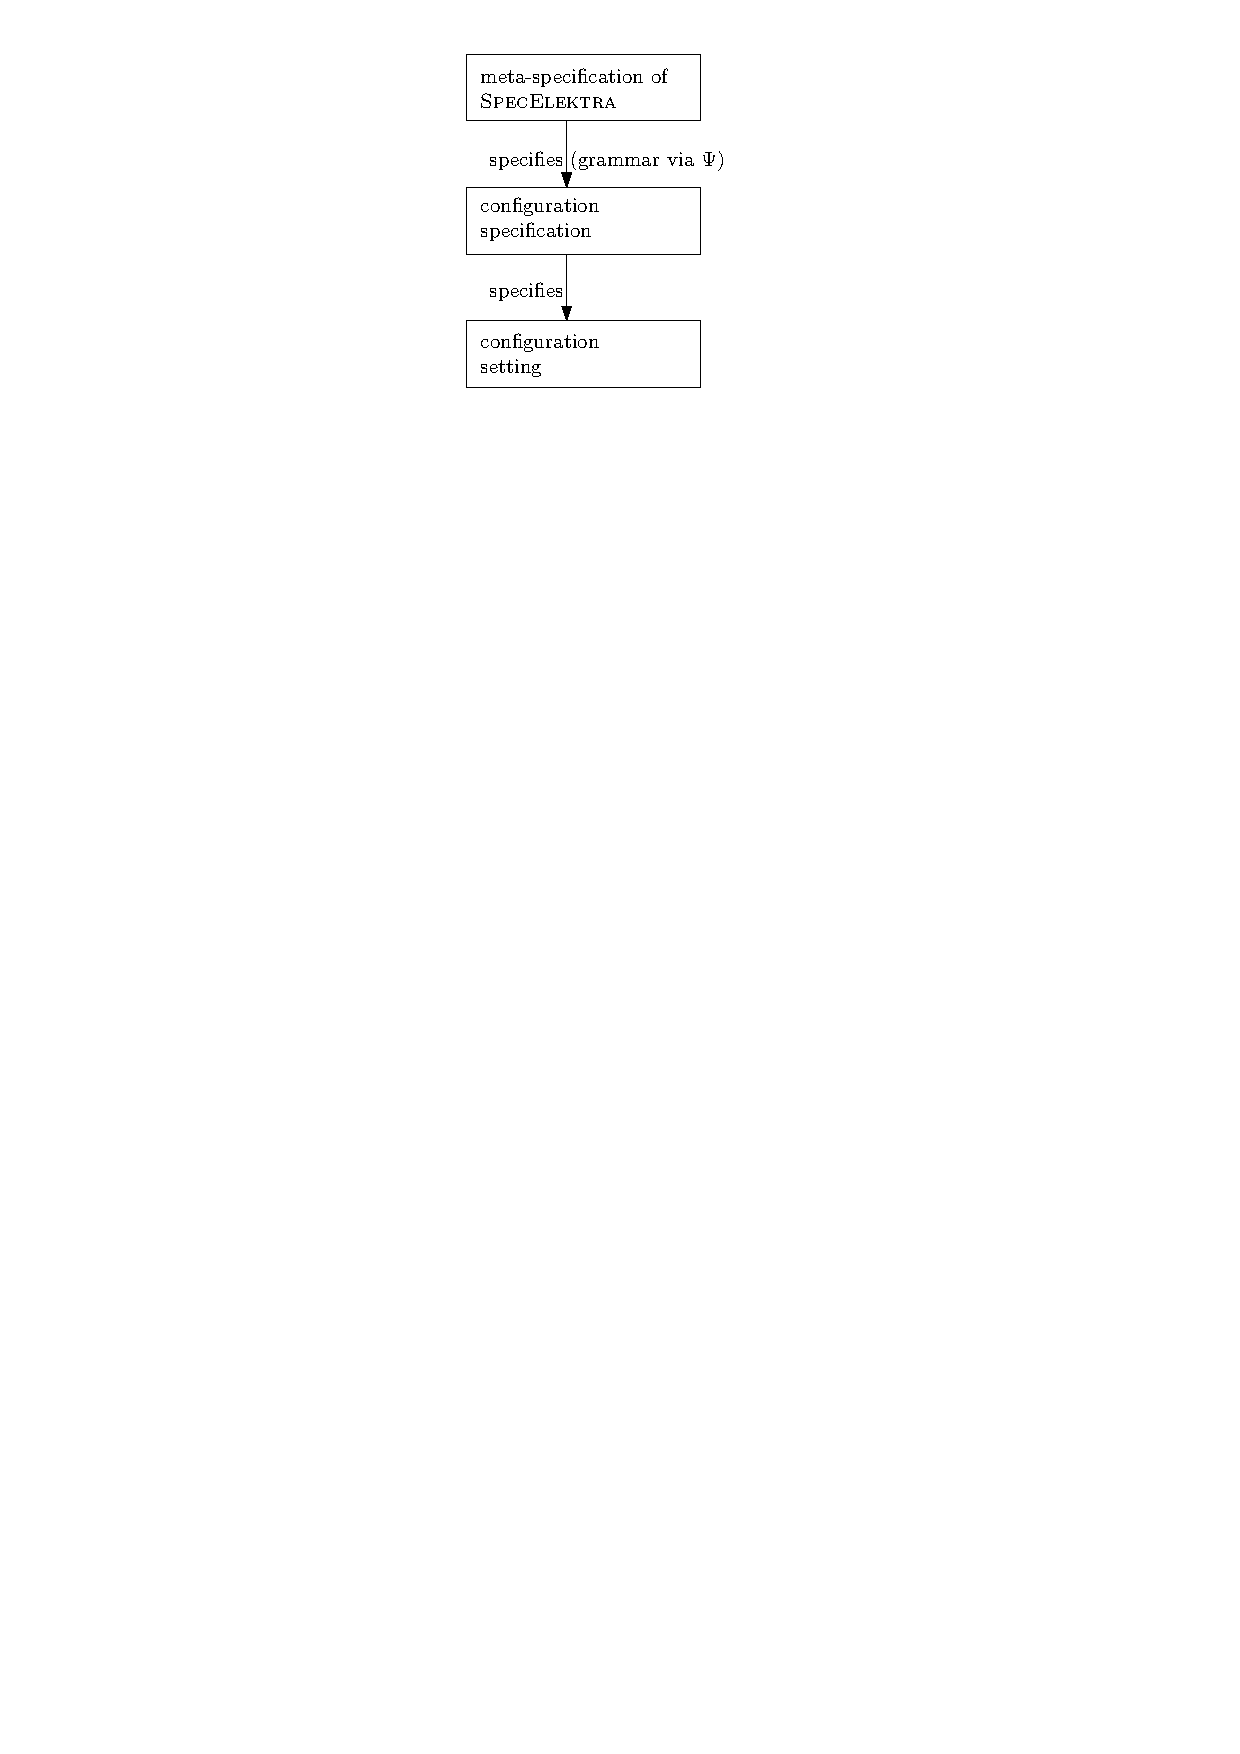
\includegraphics{metalevels}
\end{frame}

\begin{frame}
	Topic 03: \textit{Configuration Integration}
	\\ \vspace{1cm}
	art and technical challenges of sharing configurations between applications
\end{frame}


\begin{frame}
	Topic 04: \textit{Sources of Configuration}
	\begin{itemize}
		\item configuration file formats
		\item command-line arguments
		\item environment variables
	\end{itemize}
\end{frame}

\begin{frame}
	Topic 05: \textit{Configuration Management Tools}
	\begin{itemize}
		\item history
		\item Infrastructure as Code
		\item configuration drift
		\item push vs.\ pull
		\item full vs.\ partial changes
		\item examples: Puppet, Chef, Ansible, CfEngine, Nix, \dots
	\end{itemize}
\end{frame}

\begin{assignment}
	\begin{task}
	Break.
	\end{task}
\end{assignment}

\begin{frame}
	Topic 06: \textit{Strategies for Validation and Modularization}
	\begin{itemize}
		\item validation techniques
		\item modularity
		\item avoidance of dependences
	\end{itemize}
\end{frame}

\begin{frame}
	Topic 07: \textit{Strategies for Reduction of Misconfiguration}
	\begin{itemize}
		\item configuration-less systems (auto-detection)
		\item context awareness
		\item finding (un)used settings
		\item desirable properties of configuration
		\begin{itemize}
			\item self-description
			\item changeability
			\item idempotence
			\item round-tripping
		\end{itemize}
	\end{itemize}
\end{frame}

\begin{frame}
	Topic 08: \textit{Early Detection of Misconfiguration}
	\\ \vspace{1cm}
	points in time for
	\begin{itemize}
		\item configuration access
		\item validation
	\end{itemize}
\end{frame}

\begin{frame}
	Topic 09: \textit{Configuration as a User Interface}
	\begin{itemize}
		\item How system administrators work.
		\item Which user interfaces exist.
		\item How to specify configuration.
		\item How to design error messages.
	\end{itemize}
\end{frame}

\begin{frame}
	Topic 10: \textit{Design of Configuration}
	\begin{itemize}
		\item complexity reduction
		\item design aspects of configuration specification
		\item documentation of configuration
	\end{itemize}
\end{frame}


\begin{frame}
	\frametitle{Elektra}
	\hfill 
\includegraphics[width=2cm]{../figures/logo}
	\vspace{-1cm}
	\begin{itemize}
		\item Elektra is one implementation of what we \\ discuss in this lecture.
		\item Configuration management tools use Elektra.
		\item Elektra is developed at TU Wien (\url{https://libelektra.org}).
	\end{itemize}
\end{frame}

\begin{frame}
	\frametitle{Possible Benefits of CM}

	\begin{task}
	What are the goals of Configuration Management?
	\end{task}

	\pause

	\begin{itemize} %[<+-| alert@+>]
	\item Documentation, Customization, Reproducability
	\item Declarative description of the system
	\item Less configuration drift
	\item Better error handling
	\item Reusability
	\item (Resource) Abstractions
	\end{itemize}
\end{frame}

\begin{assignment}
	\frametitle{In which topics are you interested?}
	\begin{task}[1]
	Discuss topics with your partner.
	Can be new topics not mentioned before.
	\end{task}

	\begin{task}[2]
	Write down the most interesting in the shared notes.
	\end{task}
\end{assignment}





%%%%%%%%%%%%%%%%%%%%%%%%%%%%%%%%%%%%%%%%%% 
\section{Organisation}

\subsection{Preliminaries}
\begin{frame}
	\frametitle{Communication}
	\begin{itemize}
		\item TUWEL \url{https://tuwel.tuwien.ac.at/course/view.php?idnumber=194030-2021S}
		\item TISS (exam) \url{https://tiss.tuwien.ac.at/course/courseDetails.xhtml?courseNr=194030&semester=2019S}
		\item GitHub (private and public repository) \\ public: \url{https://git.libelektra.org}
		\item EMail \url{markus.raab@complang.tuwien.ac.at}
		\item before/after/during meetings
	\end{itemize}
\end{frame}

\begin{frame}
	\frametitle{Inverted Classroom}
	Meeting is every week Wednesday 09:00 - 11:00 c.t.

	\begin{itemize}
		\item always read/watch the material in advance
		\item within meetings we'll do a recapitulation
		\item and you ask questions
		\item we start off with many materials
	\end{itemize}
\end{frame}

\begin{frame}
	\frametitle{Previous Knowledge}
	\begin{itemize}
		\item Obviously \textit{no} prior knowledge about Configuration or Configuration Management necessary.
		\item If you already have experience, you can use it in your talk and assignments.
		\item You should have some understanding of software engineering and software requirements.
		\item Programming skills is a must.
	\end{itemize}
\end{frame}

\begin{frame}
	\frametitle{Programming Languages}
	Elektra supports following programming languages:
	\begin{itemize}
		\item C
		\item C++
		\item Java
		\item Rust
		\item Python
		\item Go
		\item Lua
		\item Ruby
	\end{itemize}
	You can use either of these languages.
\end{frame}

\subsection{Grades}

\begin{frame}
	You will get a grade once you submitted a PR with ``CM'' in the description.
	\vspace{1cm}

	To get a positive grade:
	\begin{itemize}
		\item All parts must be done.
		\item All parts must be positive.
	\end{itemize}
\end{frame}

\begin{frame}
	Grade is calculated from:
	\begin{description}
	\item[30\,\%:] homework
	\item[30\,\%:] team exercise
	\item[10\,\%:] talk
	\item[30\,\%:] test
	\item[+:] extrapoints
	\end{description}
\end{frame}

\subsection{Assignments}
\begin{frame}
	\frametitle{Talk}
	\begin{itemize}
		\item About anything related to configuration management.
		\item The duration must be 10--20 minutes.
		\item It must be about your experience.
		\item I.e., not only about study of literature.
		\item E.g., about:
		\begin{itemize}
			\item homework you did (e.g. H1 or T1)
			\item some CM tool you played around with
			\item some application you struggled to configure
		\end{itemize}
	\end{itemize}
\end{frame}

\begin{frame}
	\frametitle{Deadlines}

	\begin{itemize}
	\item if you make submissions earlier, you get feedback earlier
	\item dates are both in ``semester schedule.pdf'' and calender of TUWEL
	\end{itemize}

	There are always two deadlines for each homework+teamwork:

	\begin{itemize}
	\item regular deadline (submission)
	\item deadline for corrections (based on the feedback of submission but you can also extend the submission)
	\end{itemize}
\end{frame}

\begin{assignment}
	\begin{task}
	Talk with someone about a potential collaboration in the team exercise.
	\end{task}
\end{assignment}

\begin{assignment}
	\frametitle{Questions?}
	\begin{task}
	Please register for the course by doing H0.
	\end{task}

	\begin{task}
	Any questions?
	\end{task}
\end{assignment}



%%%%%%%%%%%%%%%%%%%%%%%%%%%%%%%%%%%%%%%%%% 
\nocite{raab2017introducing}

\appendix

\begin{frame}[allowframebreaks]
	\bibliographystyle{plainnat}
	\bibliography{../shared/elektra.bib}
\end{frame}

\end{document}


